\documentclass[11pt]{article}

% --------------------
% Packages
% --------------------
\usepackage[margin=1in]{geometry}
\usepackage{amsmath, amssymb, amsfonts}
\usepackage{graphicx}
\usepackage{float}
\usepackage{caption}
\usepackage{booktabs}
\usepackage{enumitem}
\usepackage{mathtools}
\usepackage{hyperref}
\usepackage{helvet}
\renewcommand{\familydefault}{\sfdefault}

\setlength{\parindent}{0in}

% --------------------
% Formatting
% --------------------
\title{Numerical PDEs Homework \#0}
\author{Hope Elsayed}
\date{9/6/26}

\begin{document}

\maketitle

% ==================================================
\section*{Problem 1: Finite Differences}
% ==================================================

Write a MATLAB code that uses finite differences to compute the first derivative of
\[
f(x) = \exp(\sin(x))
\]

on the interval $0 \leq x \leq 2\pi$. Use second-order centered differences on internal grid points and first-order one-sided differences at endpoints.

\begin{enumerate}
    \item Show a graph of the exact analytic solution $f'(x)$ and your numerical solution $f'_n(x)$. \\

\textbf{Solution:} The finite difference approximation closely follows the exact analytic derivative on the interval $0 \leq x \leq 2\pi$ as seen in Figure~\ref{fig:Q1a}. Looking closely, we can see larger errors at the endpoints because we used first-order one-sided differences instead of second-order centered differences.

\begin{figure}[H]
    \centering
    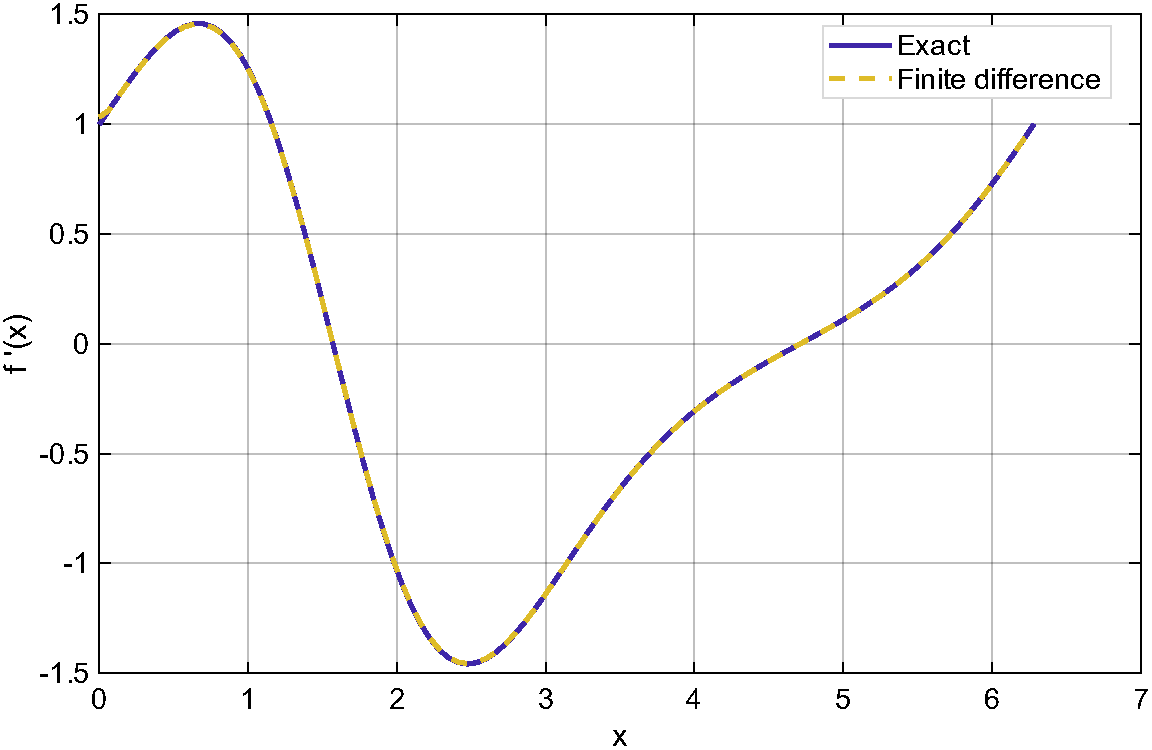
\includegraphics[width=0.8\textwidth]{Q1a.pdf}
    \caption{Exact analytic solution vs. numerical solution}
    \label{fig:Q1a}
\end{figure}
    
    \item Show a relative error convergence plot by plotting the relative error on the $y$-axis and the grid size $N$ on the $x$-axis. Measure relative error as
    \[\mathrm{Err}=
    \frac{\left\|f'(x)-f'_n(x)\right\|_p}{\left\|f'(x)\right\|_p}.
    \]

    Plot the error using both the $p=\infty$ and $p=2$ norms on a log-log scale.

    The relative errors should be lines with slopes $1$ and $3/2$, respectively; i.e., it scales with $\frac{1}{N}$ and $\frac{1}{N^{3/2}}$. \\

\textbf{Solution:} The relative errors decrease as the granularity of the grid increases. The infinity-norm slope is approximately $-1.011$, showing first-order convergence, while the 2-norm slope is approximately $-1.580$, which is close to the $-3/2$ convergence rate.

\begin{figure}[H]
    \centering
    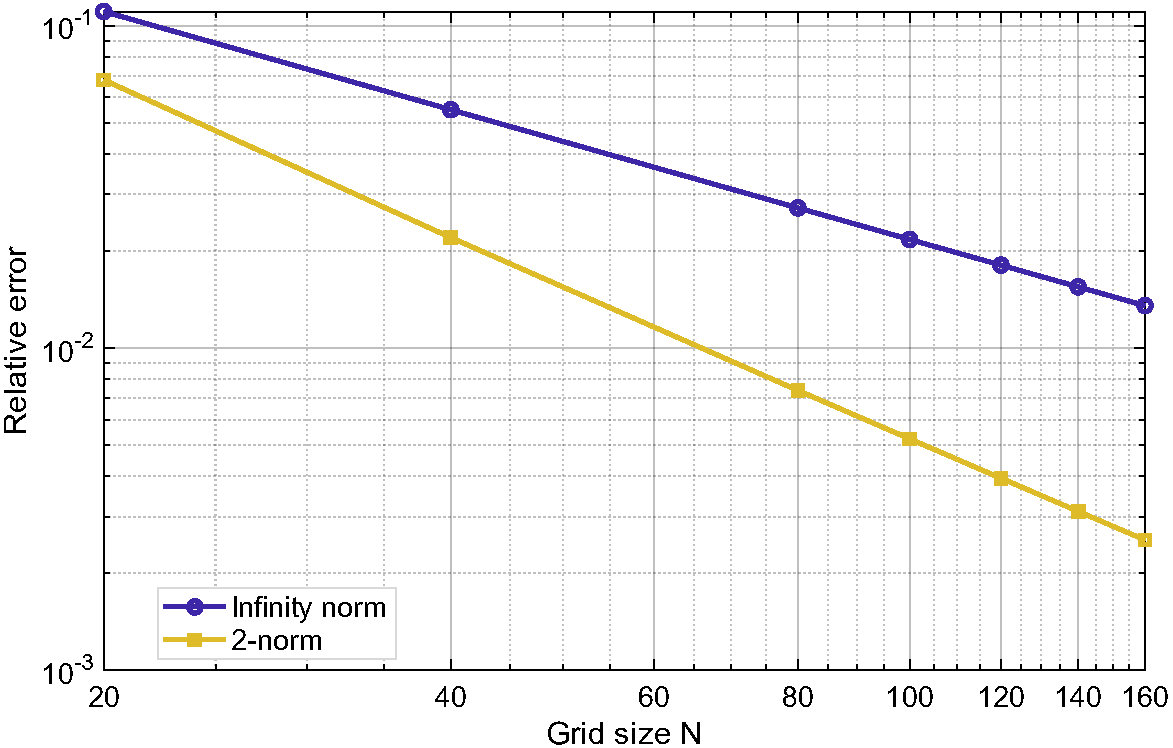
\includegraphics[width=0.8\textwidth]{Q1b.pdf}
    \caption{Relative error convergence plot}
    \label{fig:Q1b}
\end{figure}
    
    Extra Credit: The $3/2$ slope is strange. Why is that happening? \\

    \textbf{Solution: } 

The relative $2$-norm error is
\[
\mathrm{err}_2
=
\frac{\|f'-f'_n\|_2}{\|f'\|_2}
\]

$f'(x_i)\sim O(1)$ and $f'_n(x_i)\sim O(1)$ at each of the $N+1$ grid points because their values are not affected by grid spacing. 

For the denominator, we can write:
\[
\begin{aligned}
\|f'\|_2 &= \sqrt{\sum_{i=0}^{N}f'(x_i)^2} \\
&\sim \sqrt{(N+1)\cdot O(1)} \\
&\sim O(N^{1/2})
\end{aligned}
\]

For the numerator, we can write:
\[
\|f'-f'_n\|_2 = \sqrt{\sum_{i=0}^{N}(f'(x_i)-f'_n(x_i))^2} 
\]

We know that the second order approximations at the $N-1$ interior points have error $O(h^2)=O(N^{-2})$ and the first order boundary approximations at both ends have error $O(h)=O(N^{-1})$. So, we can say:

\[
\begin{aligned}
\|f'-f'_n\|_2 &\sim \sqrt{(N-1)O(N^{-2})^2+2O(N^{-1})^2} \\
&\sim \sqrt{O(N^{-3})+O(N^{-2})} \\
&\sim
O(N^{-1})
\end{aligned}
\]

Plugging in for the numerator and denominator gives:
\[
\mathrm{err}_2 \sim
\frac{O(N^{-1})}{O(N^{1/2})} \sim
\boxed{O(N^{-3/2})}
\]

Since $h=O(N^{-1})$, we can rewrite to say
\[
\boxed{\mathrm{err}_2=O(h^{3/2})}
\]
    
\end{enumerate}



\newpage
% ==================================================
\section*{Problem 2: Second-Order Derivatives}
% ==================================================

Repeat Problem 1, but compute the second derivative $f''(x)$. Assume periodicity and wrap around the grid instead of using one-sided finite differences. \\

\textbf{Solution:} The finite difference approximation closely follows the exact analytic second derivative on the interval $0 \leq x \leq 2\pi$ as seen in Figure~\ref{fig:Q2a}. Assuming periodicity allows us to use centered second-order differences at every grid point.

\begin{figure}[H]
    \centering
    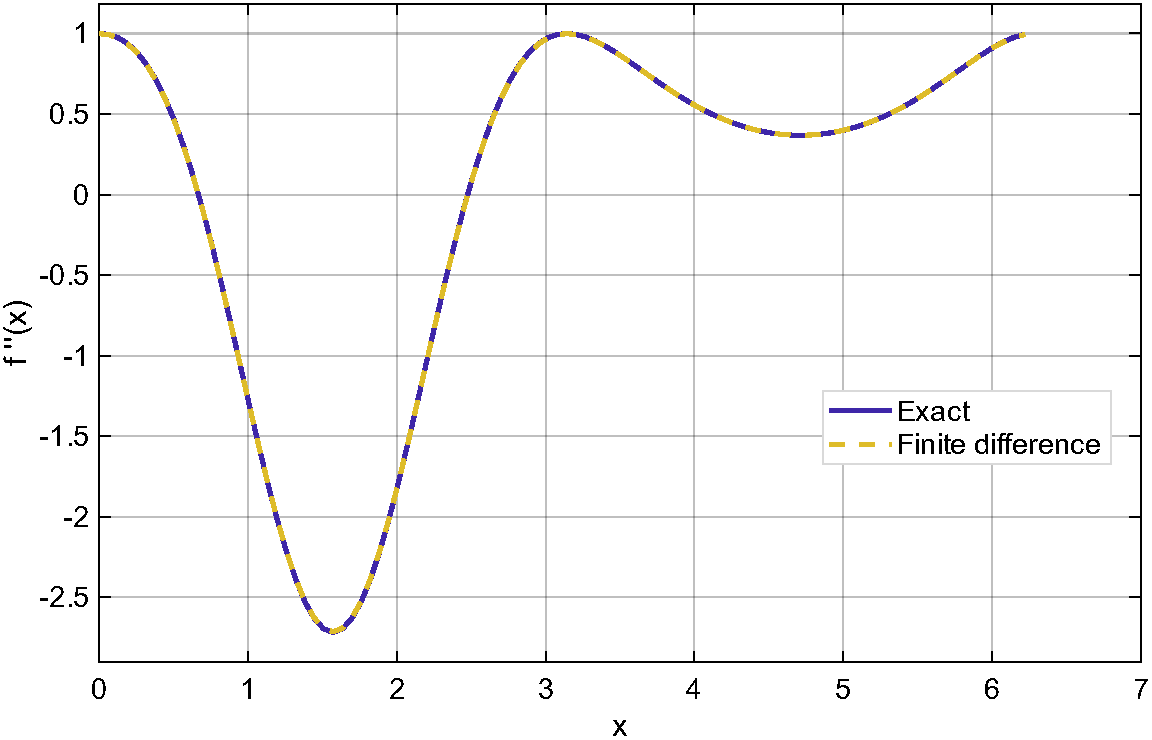
\includegraphics[width=0.8\textwidth]{Q2a.pdf}
    \caption{Exact analytic solution vs. numerical solution}
    \label{fig:Q2a}
\end{figure} 

Relative errors decrease as the grid granularity increases. The infinity-norm slope is approximately $-1.995$ and the 2-norm slope is approximately $-1.996$, which are both close to the expected slope of $-2$. Therefore, the finite difference approximation demonstrates second-order convergence. The error is $O(N^{-2})$ for both norms because we assumed periodicity and used the second-order finite difference method at every point.

\begin{figure}[H]
    \centering
    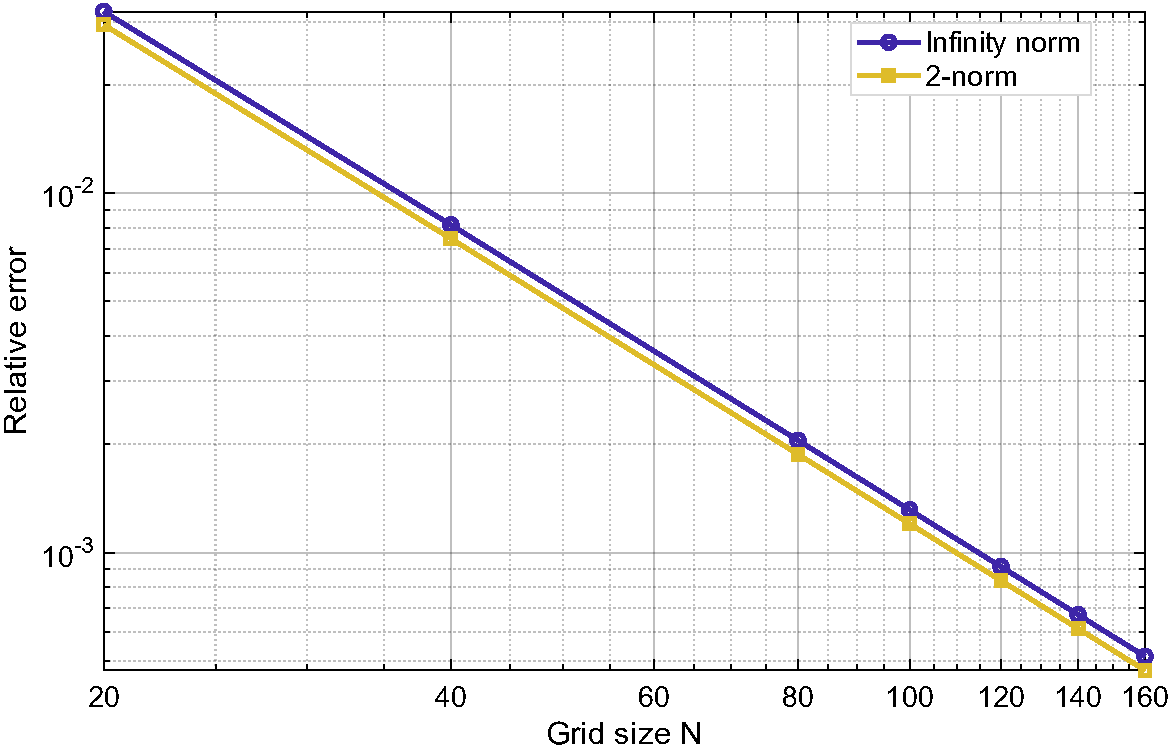
\includegraphics[width=0.8\textwidth]{Q2b.pdf}
    \caption{Relative error convergence plot}
    \label{fig:Q2b}
\end{figure}

\newpage
% ==================================================
\section*{Problem 3: ODE}
% ==================================================

Consider the ODE
\[
\frac{d^2u}{dx^2} + \sin(x)\frac{du}{dx} + u(x) = f(x)
\]

defined on $0 \leq x \leq 5$. Solve the ODE using second-order finite difference methods with Dirichlet conditions. Use $u(x)=\sin(x)$ to test your solution by finding the boundary conditions and the necessary forcing function $f(x)$. Show an error plot that proves your method converges with second order. \\

\textbf{Solution: } Using the test solution $u(x)=\sin(x)$, we have
$u'(x)=\cos(x)$, and $u''(x)=-\sin(x)$.

Substituting into $u''+\sin(x)u'+u=f(x)$ gives
\[
-\sin(x)+\sin(x)\cos(x)+\sin(x)=f(x).
\]

Therefore, $f(x)=\sin(x)\cos(x)$. The Dirichlet boundary conditions are $u(0)=\sin(0)=0$ and $u(5)=\sin(5)$. \\

The finite difference solution closely matches the exact solution $u(x)=\sin(x)$ on the interval on $0 \leq x \leq 5$ as seen in Figure~\ref{fig:Q3a}.

\begin{figure}[H]
    \centering
    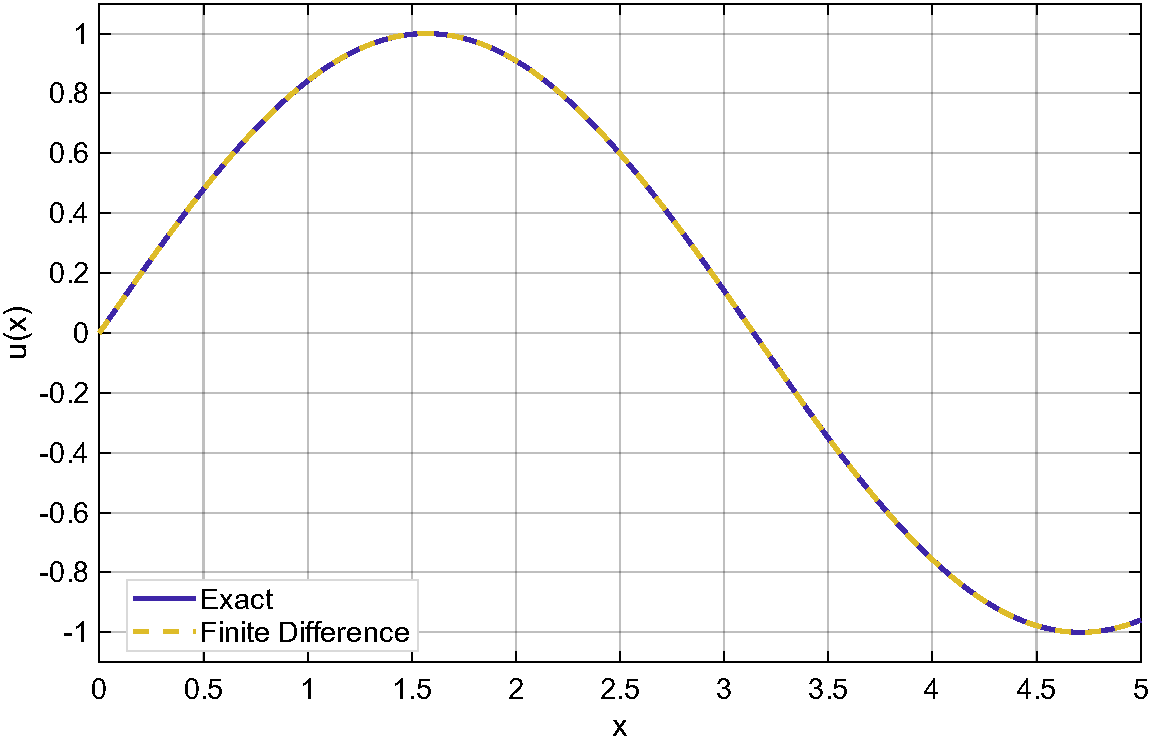
\includegraphics[width=0.8\textwidth]{Q3a.pdf}
    \caption{Exact analytic solution vs. numerical solution}
    \label{fig:Q3a}
\end{figure} 

The infinity-norm slope is approximately $-2.045$ and the 2-norm slope is approximately $-2.041$, which are both close to the expected slope of $-2$. Therefore, the finite difference approximation demonstrates second-order convergence.

\begin{figure}[H]
    \centering
    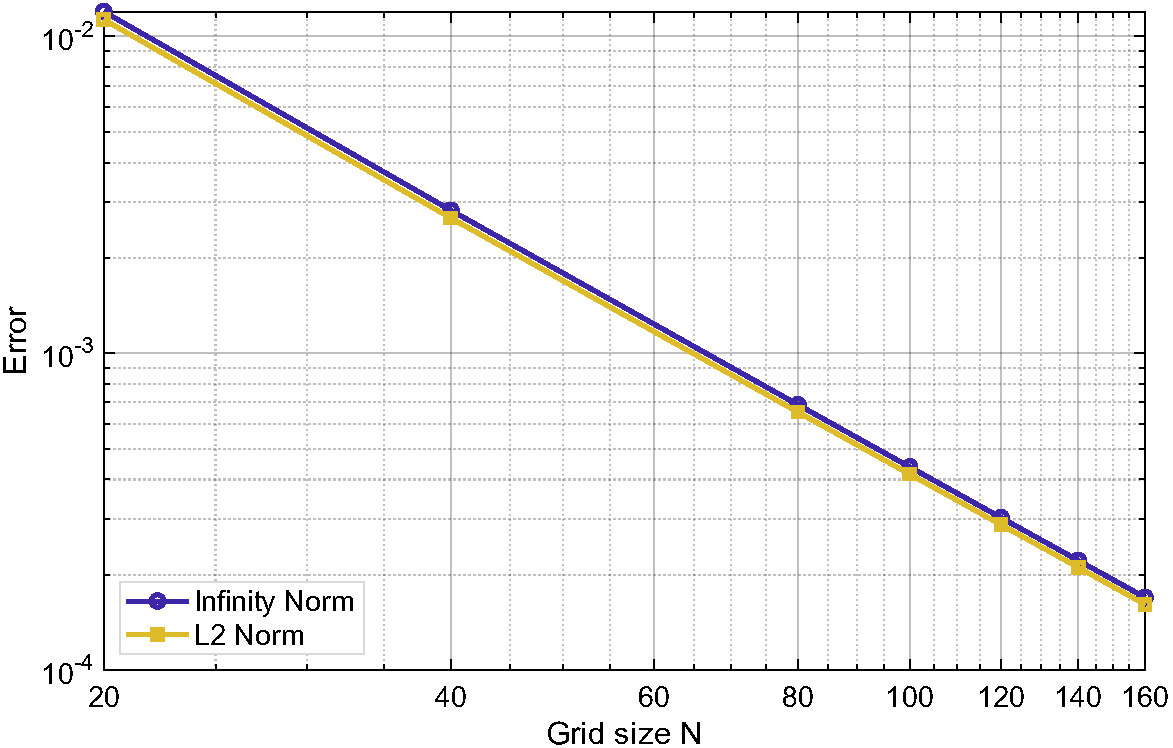
\includegraphics[width=0.8\textwidth]{Q3b.pdf}
    \caption{Relative error convergence plot}
    \label{fig:Q3b}
\end{figure} 

\newpage
% ==================================================
\section*{Problem 4: Poisson Equation}
% ==================================================

Use finite difference methods to solve the Poisson equation $\nabla^2 u = f(x,y)$ in the domain $x \in [0,5]$, $y \in [0,5]$. Use the test solution $u(x,y)=\sin(x)\cos(y)$.

\begin{enumerate}
    \item Apply Dirichlet conditions on all boundaries so that $u(x,y)$ satisfies the PDE and the boundary conditions, and show a plot of your solution and a second-order convergence plot similar to the first three problems.

\textbf{Solution: } Given that the test solution is $u(x,y)=\sin(x)\cos(y)$, the second derivatives are
\[
u_{xx}=-\sin(x)\cos(y)
\]
and
\[
u_{yy}=-\sin(x)\cos(y).
\]
Thus,
\[
\nabla^2u=u_{xx}+u_{yy}
=-2\sin(x)\cos(y) = f(x,y).
\]

The Dirichlet boundary conditions are: \\
$u(0,y)=0$

$u(5,y)=\sin(5)\cos(y)$

$u(x,0)=\sin(x)$

$u(x,5)=\sin(x)\cos(5)$ \\

We use the centered second-order finite
difference method for interior points:
\[
u_{xx}(x_i,y_j)
\approx
\frac{u_{i-1,j}-2u_{i,j}+u_{i+1,j}}{h^2},
\]
\[
u_{yy}(x_i,y_j)
\approx
\frac{u_{i,j-1}-2u_{i,j}+u_{i,j+1}}{h^2}.
\]
Adding those, we get
\[
\frac{
u_{i-1,j}+u_{i+1,j}+u_{i,j-1}+u_{i,j+1}
-4u_{i,j}}
{h^2}
=f_{i,j}.
\]

So, we have a system of equations for the interior points that we solved for. The Dirichlet boundary conditions were subtracted from the right-hand side. Figure~\ref{fig:Q4a} shows the resulting numerical solution.

\begin{figure}[H]
    \centering
    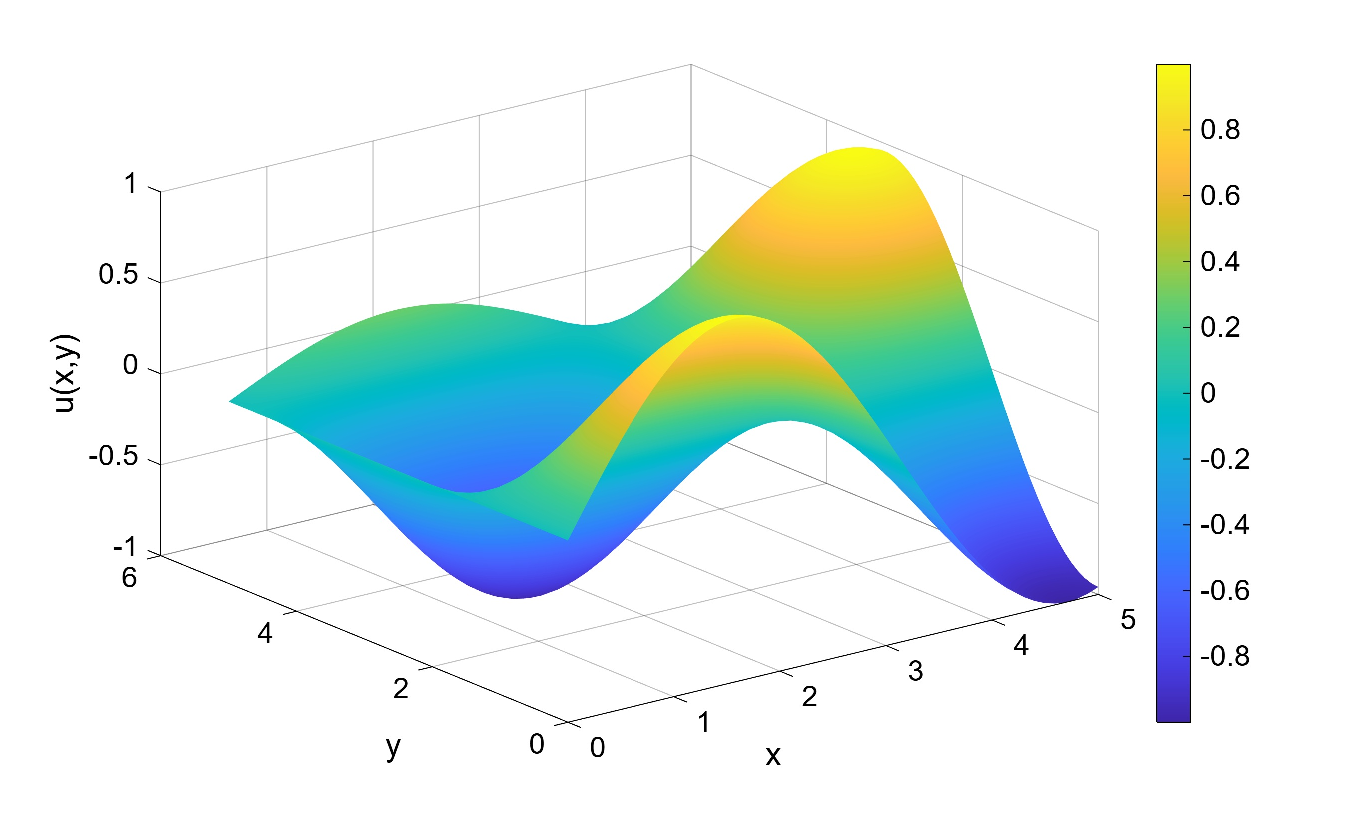
\includegraphics[width=0.8\textwidth]{Q4a.pdf}
    \caption{Numerical solution to the two-dimensional Poisson equation
    using Dirichlet boundary conditions.}
    \label{fig:Q4a}
\end{figure}


Relative errors decrease as the grid granularity increases. The infinity-norm slope is approximately $-2.043$ and the 2-norm slope is approximately $-2.023$, which are both close to the expected slope of $-2$. Therefore, the finite difference approximation demonstrates second-order convergence.

\begin{figure}[H]
    \centering
    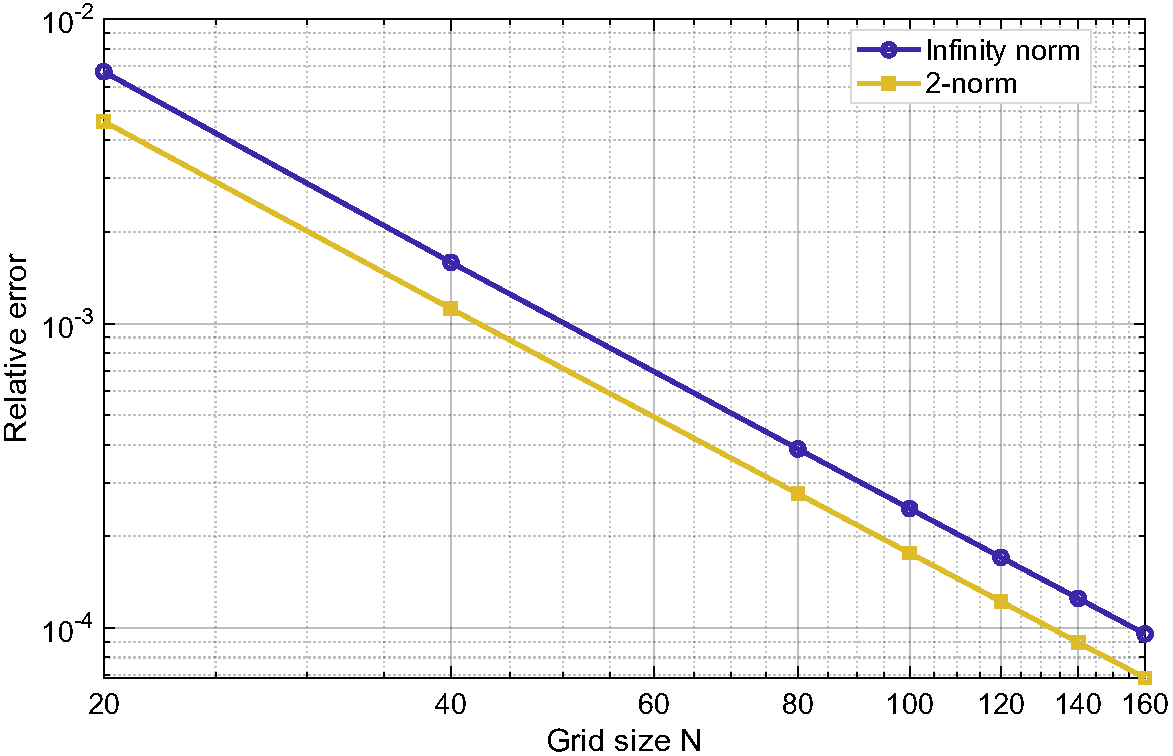
\includegraphics[width=0.8\textwidth]{Q4b.pdf}
    \caption{Relative error convergence for the finite difference
    solution. The $O(N^{-2})$ reference line indicates second-order
    convergence.}
    \label{fig:Q4b}
\end{figure}

    \item Modify your code to apply Neumann conditions on all boundaries. This won't work. Why not---both in terms of the linear algebra and in terms of the actual PDE we want to solve? Suggest a solution to the issue.

\textbf{Solution: }

With Neumann boundary conditions, the solution is not unique. If $u(x,y)$ is a solution, then for any constant $C$,
\[
\nabla^2(u+C)=\nabla^2u=f,
\]
Since the derivative of a constant is zero, we can say
\[
\frac{\partial (u+C)}{\partial n}
=
\frac{\partial u}{\partial n}.
\]
Thus, both $u$ and $u+C$ for any value of $C$ are solutions to the PDE with Neumann boundary conditions.

In terms of the linear algebra, we can write the problem as
\[
A\mathbf{u}=\mathbf{b},
\]
where $A$ is our linear system of equations, $\mathbf{b}$ is the vector of solutions, and $\mathbf{u}$ is our flattened vector of unknowns. The solution to this equation is not unique; any constant vector is in the null space of $A$ and the system does not have a unique
solution.

One solution to this problem could be to specify the value of $u$ at one point, effectively "pinning" one solution.

\end{enumerate}


\end{document}